%===============================================================================
% Zentrale Layout-Angaben und Befehle
%===============================================================================
%
% Für bessere Sicht von falschen Umbrüchen die Option draft benutzen.
% Dadurch können aber die eingebundenen Bilder nicht sichtbar sein.
\documentclass[a4paper, 12pt]{article}
%
% Hier zunächst die benötigten Packages
\usepackage{german}
\usepackage[utf8]{inputenc}
\usepackage{fancyhdr}
\usepackage[T1]{fontenc}
\usepackage{ae}
\usepackage{listings}
\usepackage{color}
\usepackage{wrapfig}
\usepackage[printonlyused]{acronym}
\usepackage{url}
\usepackage[hypertexnames=false]{hyperref}
\usepackage{fmtcount}
\usepackage[section]{placeins}
\usepackage{tabularx}
\usepackage{amsmath}
\usepackage{nameref}
%
% Einbindung des Grafik-Pakets
\ifx\pdfoutput\undefined
	\usepackage[dvips]{graphicx}
\else
	\usepackage[pdftex]{graphicx}
\pdfcompresslevel=9
\pdfpageheight=297mm
\pdfpagewidth=210mm
\fi
\usepackage[colorinlistoftodos,prependcaption,textsize=tiny]{todonotes}
%
% Page-Layout
\setlength\headheight{14pt}
\setlength\topmargin{-15,4mm}
\setlength\oddsidemargin{-0,4mm}
\setlength\evensidemargin{-0,4mm}
\setlength\textwidth{160mm}
\setlength\textheight{252mm}
%
% Absatzeinstellungen
\setlength\parindent{0mm}
\setlength\parskip{2ex}
%
% dont break math space
\binoppenalty=10000
\relpenalty=10000
%
% Kopf- und Fusszeile
\pagestyle{fancy}
\fancyhf{} % alles löschen
\fancyhead[LO]{\footnotesize\sc\nouppercase{\leftmark}}
\fancyfoot[LO]{\footnotesize\sc Lehrstuhl f\"ur Praktische Informatik}
\fancyfoot[RO]{\thepage}
\renewcommand{\headrulewidth}{0pt}
\renewcommand{\footrulewidth}{0pt}
%
% Bessere Fehlermeldungen
\errorcontextlines=999
%
% Anweisung zur Erstellung der Titelseite
% #1 Bachelorarbeit || Masterarbeit
% #2 = Studiengang
% #3 = Titel der Arbeit
% #4 = Autor
% #5 = Abgabedatum
\renewcommand{\maketitle}[6]
{
\pagenumbering{Alph}
\begin{titlepage}
\centering
\begin{minipage}[t]{16cm}
\begin{minipage}{3cm}
    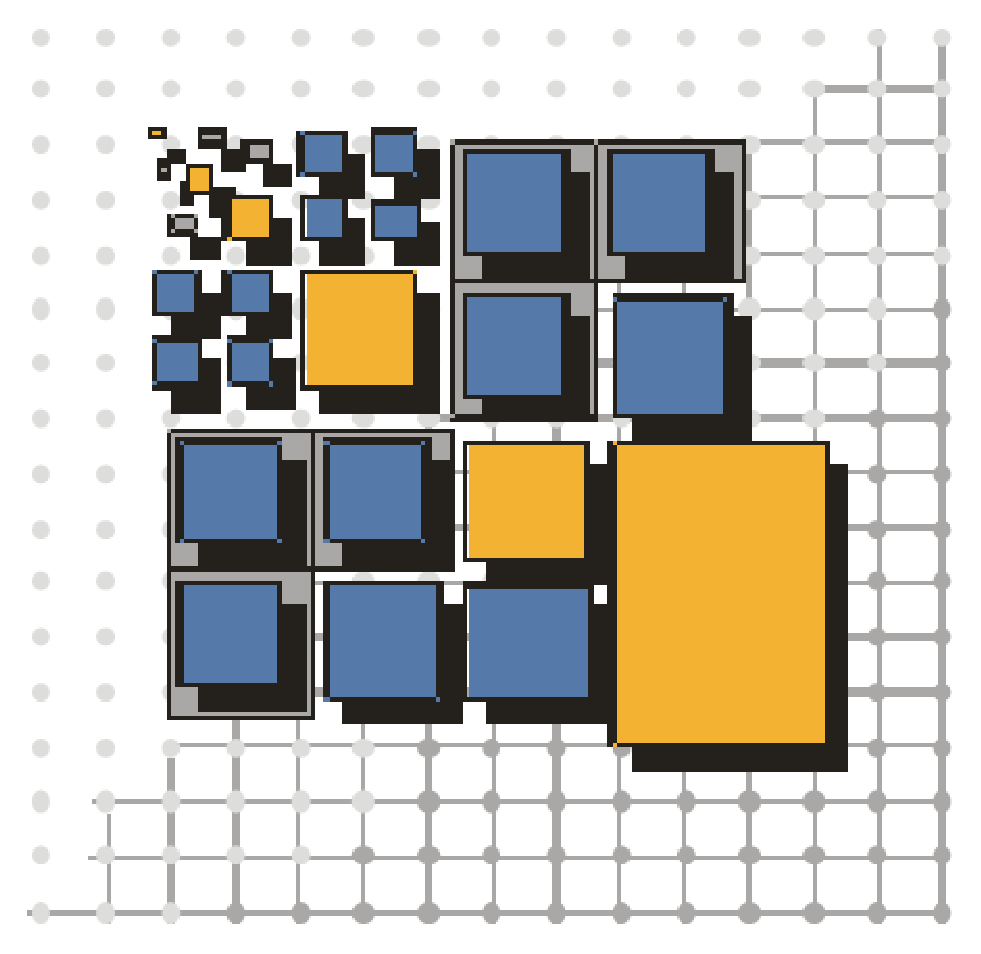
\includegraphics[height=26mm]{includes/vs-logo}
\end{minipage}
\hfill
\begin{minipage}{9cm}
  \centering
    Otto-Friedrich-Universit\"at Bamberg\\[12pt]
    {\Large Lehrstuhl f\"ur Praktische Informatik}
\end{minipage}
\hfill
\begin{minipage}{3cm}
    
\includegraphics[height=26mm]{includes/UB-Logo-neu_blau-cmyk}
\end{minipage}
\end{minipage}\\[130pt]
{\LARGE #1}\\[124pt]
Zum Thema:\\[24pt]
{\Huge #2}\\[60pt]
\vfill
\begin{minipage}{\textwidth}
\center
Vorgelegt von:\\
{\Large #3\\[12pt]}
Betreuer:\\
{#5\\[12pt]}
Themensteller:\\
#6\\[12pt]
Abgabedatum:\\
#4\\
\end{minipage}
\end{titlepage}
}

%
% Wird für Hintergrund von Codelistings benötigt
\definecolor{hellgrau}{gray}{0.9}
%
\lstdefinelanguage{JavaScript}{
	keywords={typeof, new, true, false, catch, function, return, null, catch, switch, var, if, in, while, do, else, case, break},
	ndkeywords={class, export, boolean, throw, implements, import, this},
	sensitive=false,
	comment=[l]{//},
	morecomment=[s]{/*}{*/},
	morestring=[b]',
	morestring=[b]"
}
% Einstellungen für Java-Code
\lstdefinestyle{javaStyle}{%
	basicstyle=\small,%
	backgroundcolor=\color{hellgrau},%
	keywordstyle=\bfseries,%
	showstringspaces=false,%
	numbers=left,%
	numberstyle=\footnotesize,%
	stepnumber=1,%
	numbersep=3pt,%
	extendedchars=true,%
	xleftmargin=2em,%
	lineskip=-1pt,%
	tabsize=4,%
	language=Java,
	breaklines,%
	identifierstyle=\ttfamily,
}
% set default to java, explicitly set to others when needed
\lstset{style=javaStyle}
%
% neues environment für Java-Sourcecode
% #1 = "caption={Hier eigene Überschrift}, label={Hier eigenes Label}"
\lstnewenvironment{javacode}[1][]{%
\lstset{style=javaStyle,#1}%
}{}
%
% Befehl zum Einbinden von Java-Sourcecode aus Datei
% #1 = Dateiname relativ zu src-Verzeichnis
% #2 = Überschrift
% #3 = Label
\newcommand{\javafile}[3]{%
   \lstinputlisting[%
     caption={#2},%
     label={#3},%
     style=javaStyle,
     captionpos=b]{src/#1}%
}
%
% Einbindung eines Bildes
% #1 = Name des Bildes ohne Endung relativ zu images-Verzeichnis
% #2 = Caption
% #3 = label für \ref-Verweise
% #4 = Breite des Bildes im Dokument in % der breite
\newcommand{\asfigure}[4]{%
  \begin{figure}[htb]%
    \begin{center}%
      \includegraphics[width=#4\textwidth]{images/#1}%
      \vskip -0.3cm%
      \caption{#2}%
      \vskip -0,2cm%
      \label{#3}%
    \end{center}%
  \end{figure}%
}
%
% Umgebung für Fliesstext um Grafik
% #1 = Ausrichtung: r, l, i, ...
% #2 = Breite des Bildes in cm
% #3 = Name des Bildes ohne Endung relativ zu images-Verzeichnis
% #4 = Beschriftung
% #5 = label für \ref-Verweise
\newcommand{\textflow}[5]{%
\begin{wrapfigure}{#1}{#2cm}%
\includegraphics[width=#2cm]{images/#3}%
\caption{#4}%
\label{#5}%
\end{wrapfigure}%
}
%%%
\makeatletter
\let\orgdescriptionlabel\descriptionlabel
\renewcommand*{\descriptionlabel}[1]{%
	\let\orglabel\label
	\let\label\@gobble
	\phantomsection
	\edef\@currentlabel{#1}%
	%\edef\@currentlabelname{#1}%
	\let\label\orglabel
	\orgdescriptionlabel{#1}%
}
\makeatother

%%% Local Variables:
%%% mode: latex
%%% TeX-master: t
%%% End:

\usepackage{listings}
%
% Backgroundcolor
\definecolor{hellgrau}{gray}{0.9}
%
% Configuration
%
\lstdefinestyle{javaStyle}{%
	basicstyle=\small,%
	backgroundcolor=\color{hellgrau},%
	keywordstyle=\bfseries,%
	showstringspaces=false,%
	numbers=left,%
	numberstyle=\footnotesize,%
	stepnumber=1,%
	numbersep=3pt,%
	extendedchars=true,%
	xleftmargin=2em,%
	lineskip=-1pt,%
	tabsize=4,%
	language=Java,
	breaklines,%
	identifierstyle=\ttfamily,
}
%
% Java-Sourcecode environment
% #1 = Caption
% #2 = Label
%
\lstnewenvironment{javacode}[2]%
{\lstset{style=javaStyle,caption=#1,label=#2}}
{}
% Include code from Java-file
% #1 = Filename relative to section-folder
% #2 = Caption
% #3 = Label
%
\newcommand{\javafile}[3]{%
   \lstinputlisting[%
     caption={#2},%
     label={#3},%
     style=javaStyle]{src/#1}%
}

%
\begin{document}
%
% Create title page
\maketitle{Seminar Topic}{LaTeX only}%
{Author}{Prof. Dr. Guido Wirtz}{Winterterm 2018/2019}{Bachelor|Master}
%
% Create lists of content
\pagenumbering{Roman}
\tableofcontents
\newpage
\listoffigures
\newpage
\listoftables
\newpage
\lstlistoflistings
\newpage
%
% Abkürzungen
%
\section*{Abkürzungsverzeichnis}
% In Klammern steht das längste Akronym!
\begin{acronym}[LSPI]
 \acro{DSG}{Distributed Systems Group}
 \acro{LSPI}{Lehrstuhl für Praktische Informatik}
\end{acronym}
\newpage
\setcounter{page}{1}
\pagenumbering{arabic}
%
% Include sections with \input{section-file}
%
%
\section{Einleitung}
%
Zur Verfassung von Seminar-, Bachelor- und Masterarbeiten bietet die Distributed Systems Group
neben den Word-Vorlagen auch Vorlagen für Latex. In diesem Dokument soll
kurz gezeigt, wie die einzelnen Umgebungen und Befehle der Vorlage sinnvoll zur Erstellung
von Arbeiten genutzt werden können. Es erfolgt aber keine allgemeine Anleitung zur
Erstellung von Dokumenten mit \LaTeX. Als Einstiegsliteratur, die aber für die allgemeine
Arbeit mit \LaTeX~durchaus ausreichend ist, eignet sich das Buch von Kopka \cite{kop02}. Eines
der älteren Werke des Autors reicht ebenfalls aus. 
Eine sehr gute Übersicht über alle wichtigen Szenarien gibt das Wikibook "`\LaTeX"' \cite{lat12}.
Weitere hilfreiche Lektüre findet sich
unter \cite{jue00}, \cite{kue11}, \cite{jue95}, \cite{erb09} und allen verfügbaren Suchmaschinen.

Die Erstellung eines \LaTeX-Dokumentes erfolgt z.B. über die Anweisung \texttt{pdflatex seminar} oder mit einer 
entsprechenden IDE, wie \textit{TeXnicCenter}\footnote{\url{http://www.texniccenter.org}} oder \textit{TeXlipse}\footnote{\url{http://texlipse.sourceforge.net}}.
Hier empfiehlt sich auch das Zusammenspiel mit SumatraPDF\footnote{\url{http://blog.kowalczyk.info/software/sumatrapdf/free-pdf-reader-de.html}}, das eine Vorwärts- und Rückwärtssuche in den Dokumenten ermöglicht. 
%
%
\section{General structure}
%
The central file of the template is \texttt{seminar.tex} which needs to be adjusted by the specific author for a specific thesis.
In the file, settings for the title page can be changed.
Furthermore, the files for the individual sections need to be included, as well as the \textit{.bib}-file containing \textit{bibtex}-entries.
%
\subsection{Creation of a title page}
%
A title page can be created using the command \texttt{\textbackslash maketitle}. 
Depending on whether it is a seminar paper or a Bachelor/Masterthesis, the command has a different number of parameters. 
To create a title page for a seminar paper, six parameters need to be passed to \texttt{\textbackslash maketitle}.
%
\begin{verbatim}
\maketitle{Seminar topic}{Paper topic}%
{Author}{Supervisor}{Semester}{Bachelor|Master}
\end{verbatim}
%
The individual parameters are self-explanatory.
If the seminar paper is written by more than one author, the names should be separated by \texttt{,\textbackslash\textbackslash}.
In the case of three authors, the third parameter would therefore be  \texttt{Hans Meier,\textbackslash\textbackslash\ Peter Müller and\textbackslash\textbackslash\ Hans Müller} as an example.
For the semester, an abbreviation should be used, such as \texttt{SoSe19}.

To create a title page for a Bachelor/Masterthesis, the command \texttt{\textbackslash maketitle} has to be called with three parameters.
%
\begin{verbatim}
\maketitle{Bachelor-/Masterthesis}{Course of studying}{Thesis topic}%
{Author}{Submission date}
\end{verbatim}
%
Also in this case, the parameters are self-explanatory.
%
\subsection{Including sections}
%
To keep the work well-arranged, it is reasonable to create a \textit{.tex}-file for each section.
To assemble the files to one single document, the sections need to be included using the command  \texttt{\textbackslash input} inside the file \texttt{seminar.tex}.
If, for example, a section should be included which is inside the file \texttt{section-1.tex}, then the following command would be used:

\texttt{\textbackslash input\{section-1\}}

%
\subsection{Including the bibliography}
%
The literature sources should be listed in a \textit{.bib}--file.
The \textit{bibtex}--file \texttt{example.bib} contains some examples of different sources, like books, articles, etc.
Each entry needs a unique label, which is formed from the first three letters of the lastname of the author and the last two digits of the year when it was published.
If there is more than one author for a source, the label is formed from the beginning letters of the lastnames of the first three authors and the last two digits of the year when it was published.
If an author has published more than one work within a year, the following labels should be appended with small letters, starting with \textit{b}.

A \textit{.bib}-file should be included using \texttt{\textbackslash bibliography} within the file \texttt{seminar.tex}.
The exemplary file \texttt{references.bib} was therefore included using:

\texttt{\textbackslash bibliography\{references\}}
%
%
\section{Including graphics}
%
Generally, graphics are included between paragraphs.
Another option is to surround graphics with text.
Graphics should be provided as or \emph{pdf} or \emph{eps}-files.
This depends on whether \emph{latex} or \emph{pdflatex} is used to create the document.
If \emph{latex} is used, only \emph{eps}-files can be included.
If the document is created with \emph{pdflatex}, \emph{pdf}-files should be used.

Graphics should be inside the \emph{images}-directory, to easily include them. 
Newly created graphics should therefore be copied to the \emph{images}-directory.

\subsection{Graphics between paragraphs}
%
Graphics can be included between paragraphs using 
\texttt{\textbackslash bild}.
\begin{verbatim}
\bild{picture1}{vs-logo}{DSG-Logo}{5}
\end{verbatim}
The first parameter \texttt{picture1} serves as a label to reference the graphic. 
The second parameter is the name of the graphics file without its file ending.
As a third parameter, the caption has to be provided and the last parameter defines the width of the graphic in centimeters. 
The width has to be provided as a numeric value. 
If a graphic is wider than the provided width, it is shrinked.
Smaller graphics are scaled up.
The above command leads to figure \ref{picture1}.

\bild{picture1}{vs-logo}{DSG-Logo}{5}

\subsection{Graphics surrounded by text}
%
If a graphic should be surrounded by text, the command \texttt{\textbackslash fliesstext} has to be used.
This command is based on the package \emph{wrapfig} which might have to be installed.
\fliesstext{r}{3}{vs-logo}{DSG-Logo}{picture2}
This package is, similar to all other environments with this functionality, limited and partially erroneous.
Therefore it should be used only with caution.
A graphic can be included with:\\\\
\verb+\fliesstext{r}{3}{vs-logo}{DSG-Logo}{picture2}+\\\\
After this command, the text follows which should surround the figure.
For the first parameter, only the small letters \emph{l} and \emph{r} are possible.
They lead to the graphic being arranged on the left or right side.
The second parameter can be used to specify the desired width in centimeters.
The graphic is scaled accordingly.
The third parameter is the name of the graphics file without its file ending.
The fourth parameter defines the caption for the figure and with the fifth parameter, a label can be defined to reference the figure.

A peculiarity of this package is that graphics are always placed at the beginning of a paragraph.
If a graphic should be enclosed completely by a paragraph, as it is the case with figure \ref{picture2}, the command 
\texttt{\textbackslash fliesstext} should not be placed before the paragraph but within it.
The above command is therefore placed after the word "`installed"'.
%
%
%
\section{Including Java source code}
%
To include Java source code, the package \emph{listings} is required, which might have to be installed.
This package enables the inclusion of source code from various programming languages into the document.
There are two possibilities to include source code in a document. 
One possibility is to put the source code directly in the document and the other is to read it from a file.

To include source code directly, a special environment is required which is shown in the following example:

\begin{verbatim}
\begin{javacode}{This is the first listing}{listing1}
public class Test{

  public Test(){
    // do something
  }

}
\end{javacode}
\end{verbatim}
%
First, an environment called \texttt{javacode} is created.
Required parameters are a caption and a label.
Then follows the actual source code and the environment is closed again.
The above example leads to listing \ref{listing1}.

\begin{javacode}{This is the first listing}{listing1}
public class Test {

  public Test(){
    // do something
  }

}
\end{javacode}

As an alternative, the source code can also be read from a file.
This is beneficial, because it increases the readability.
To include source code from a file, the command \texttt{\textbackslash javafile} is used. 
For a successful inclusion, the source code file has to be located in the \texttt{src}-directory. 

Example usage:
\begin{verbatim}
\javafile{src.java}{This is the second listing}{listing2}
\end{verbatim}

The first parameter has to be the name of the file (with file ending) inside the \emph{src}--directory.
The second parameter defines the caption and the third parameter is the label for referencing the listing.

The above example leads to listing \ref{listing2} as a result.

\javafile{src.java}{This is the second listing}{listing2}
%
%
\section{Nutzung des Abkürzungsverzeichnisses}
%
Zur Einbindung des Abkürzungsverzeichnisses wird das \texttt{acronym}--Package\footnote{\url{http://www.ctan.org/tex-archive/macros/latex/contrib/acronym}} verwendet.
Der Eintrag aller verwendeten Abkürzungen erfolgt in der Datei \texttt{abbreviations.tex}, die bspw. den folgenden Inhalt hat:
%
\begin{verbatim}
	\begin{acronym}[LSPI]
	 \acro{DSG}{Distributed Systems Group}
	 \acro{LSPI}{Lehrstuhl für Praktische Informatik}
	\end{acronym}
\end{verbatim}
%
Die geklammerte Abkürzung \texttt{[LSPI]} sollte dabei durch die längste vorhandene Abkürzung ersetzt werden.
Eine Abkürzung wird mit dem Befehl \texttt{\textbackslash acro} innerhalb der \texttt{acronym}--Umgebung definiert.
Standardmäßig werden nur die im Text tatsächlich verwendeten Abkürzungen auch im Verzeichnis ausgegeben.
Um eine Abkürzung innerhalb eines Textes einzufügen genügt der folgende Ausdruck:

\texttt{\textbackslash ac\{}\textit{<acronym>}\texttt{\}}

Bei der ersten Verwendung innerhalb des Textes bewirkt die Anweisung, dass der vollständige Name gefolgt von der Abkürzung in Klammern ausgegeben wird.
Bei jeder weiteren Verwendung wird lediglich die Kurzform ausgegeben. Die Anweisung \texttt{\textbackslash ac\{DSG\}} erzeugt also zunächst die Langform "`\ac{DSG}"'.
Anschließend nur noch die Abkürzung "`\ac{DSG}"'.
\newpage
%
% Settings for bibliography
\addcontentsline{toc}{section}{\bibname}
\bibliographystyle{IEEEtran}
%
% Include bib-file
\bibliography{bibliography/references}
\end{document}
